
\section{Generative Adversarial Networks (GAN)}

The GAN approach to generative modeling is unlike traditional approaches (PixelRNN, PixelCNN, VAE, etc.) in that its goal is not to find $P_\theta$. Rather, the goal is to find a function $G$ such that $G(z) \sim P_\theta, z \sim P_z~$ where $P_z$ is a \textit{previously known} probability distribution. In other words, GANs try to find a function that \textit{transforms} samples from a known distribution $P_z$ into samples from the target distribution $P_\theta$. We never actually find $P_\theta$, but that doesn't really matter since we are still able to draw samples from it. 

In the GAN architecture, two neural networks, a generator ($G$) and a discriminator ($D$) compete against each other (Figure \ref{fig:gan}). A common analogy for their relationship is that of a banker and a counterfeiter. The banker's goal is to discriminate between real and fake money while the counterfeiter's goal is to trick the banker into classifying his fake money as real. By participating in this game, the banker gets better at identifying fake money, and the counterfeiter gets better at manufacturing realistic fake money. In GANs, $G$ and $D$ play a similar game with each other until the samples generated by $G$ are so realistic enough that $D$ is forced to guess (with a 50\% chance of being correct) whether or not the sample is authentic. This can be formalized as a min-max game:

\begin{align}
	\label{eq:minmax}
	\underset{G}{min}~\underset{D}{max} L(D, G) =& \mathbb{E}_{x \sim P_r}~log(D(x)) + \mathbb{E}_{z \sim P_z}~log(1-D(G(z))) \\
	=& \mathbb{E}_{x \sim P_r}~log~D(x) + \mathbb{E}_{x \sim P_\theta}~log~D(1-x)
\end{align}

In other words, $D$ tries to \textit{maximize} the expected value for $log(D(x))$ over $x \sim P_r$ and $log(1-D(x))$ over $x \sim P_\theta$. At the same time, $G$ tries to \textit{minimize} the expected value of $log(1-D(x))$ over $x \sim P_\theta$. The solution to the game is a Nash Equilibrium and occurs when $D(x)=\frac{1}{2}$. We can derive this solution by finding the solution to $\frac{d f}{d D(x)} = 0$ where $f(D(x)) = P_r(x) log(D(x)) + P_\theta log(1-D(x)) = 0$, and considering the solution $P_r = P_\theta$: 

\begin{align*}
	\label{eq:optD}
	\frac{d L}{d D(x)} =& \frac{P_r(x)}{D(x)} + \frac{P_\theta * -1}{1-D(x)} \\
	0 =& \frac{P_r(x)}{D(x)} - \frac{P_\theta}{1-D(x)} \\
	P_\theta D(x) =& P_r(x) (1-D(x)) \\
	P_\theta D(x) =& P_r(x)-P_r(x) D(x) \\
	D(x)(P_\theta + P_r(x)) =& P_r(x)\\
	D(x) =& \frac{P_r(x)}{P_\theta + P_r(x)}\\
\end{align*}

Clearly, $P_r = P_\theta \Rightarrow D(x) = \frac{1}{2}$. Intuitively, this implies that the Generator's samples are so realistic that the Discriminator is forced to guess (with a 50\% chance of being correct) about their authenticity. 

\begin{figure}[h!]
	\centering
	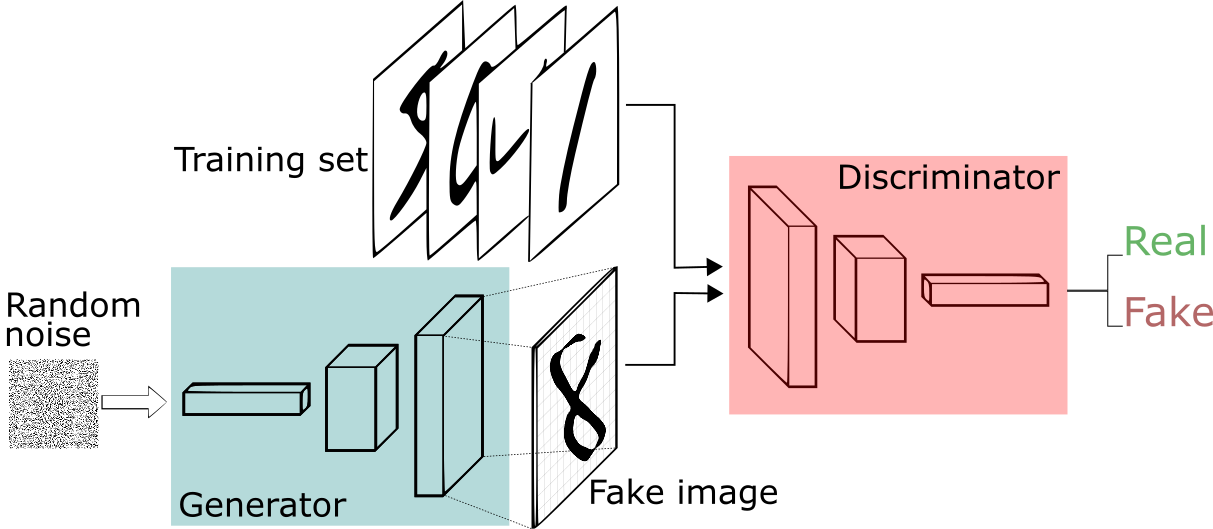
\includegraphics[width=\linewidth]{media/gan.png}
	\caption{GAN Architecture. The Discriminator receives samples from the dataset and the generator and must accurately label them as real or fake.}
	\label{fig:gan}
\end{figure}

As an implementation detail, on the generator side, minimizing $-log~D(G(z))$ (or maximizing $log~D(G(z))$) is better than minimizing $log~D(1-G(z))$ since it's gradients are better for initial samples generated by $G$.

So for the discriminator, we want to maximize:

\begin{equation}
	\label{eq:maxD}
	\mathbb{E}_{x \sim P_r}~log~D(x) + \mathbb{E}_{z \sim P_z} log D(1-G(z))
\end{equation}

and for the generator, we want to maximize:

\begin{equation}
	\label{eq:maxG}
	\mathbb{E}_{z \sim P_z}~log~D(1-G(z))
\end{equation}

\subsection{Problems with GAN}
Since $D$ and $G$ are neural networks, we can maximize them with using Stochastic Gradient Descent. Since we are training two networks simealtaneously, finding an equilibrium that optimizes both functions is difficult. Also, the fact that images appear to be high-dimensional hundreds of pixels, studies show they are actually low-dimensional. Intuitively, we can think about how objects in an image are extremely dependent each other. For example, a picture of a person always contains two eyes relatively the same distance apart. KL-Divergence and Jenson-Shannon Divergence do not support low-dimensional manifolds well. 